% Options for packages loaded elsewhere
\PassOptionsToPackage{unicode}{hyperref}
\PassOptionsToPackage{hyphens}{url}
\PassOptionsToPackage{dvipsnames,svgnames,x11names}{xcolor}
%
\documentclass[
]{report}

\usepackage{amsmath,amssymb}
\usepackage{iftex}
\ifPDFTeX
  \usepackage[T1]{fontenc}
  \usepackage[utf8]{inputenc}
  \usepackage{textcomp} % provide euro and other symbols
\else % if luatex or xetex
  \usepackage{unicode-math}
  \defaultfontfeatures{Scale=MatchLowercase}
  \defaultfontfeatures[\rmfamily]{Ligatures=TeX,Scale=1}
\fi
\usepackage{lmodern}
\ifPDFTeX\else  
    % xetex/luatex font selection
\fi
% Use upquote if available, for straight quotes in verbatim environments
\IfFileExists{upquote.sty}{\usepackage{upquote}}{}
\IfFileExists{microtype.sty}{% use microtype if available
  \usepackage[]{microtype}
  \UseMicrotypeSet[protrusion]{basicmath} % disable protrusion for tt fonts
}{}
\makeatletter
\@ifundefined{KOMAClassName}{% if non-KOMA class
  \IfFileExists{parskip.sty}{%
    \usepackage{parskip}
  }{% else
    \setlength{\parindent}{0pt}
    \setlength{\parskip}{6pt plus 2pt minus 1pt}}
}{% if KOMA class
  \KOMAoptions{parskip=half}}
\makeatother
\usepackage{xcolor}
\usepackage[top=30mm,left=20mm]{geometry}
\setlength{\emergencystretch}{3em} % prevent overfull lines
\setcounter{secnumdepth}{-\maxdimen} % remove section numbering
% Make \paragraph and \subparagraph free-standing
\ifx\paragraph\undefined\else
  \let\oldparagraph\paragraph
  \renewcommand{\paragraph}[1]{\oldparagraph{#1}\mbox{}}
\fi
\ifx\subparagraph\undefined\else
  \let\oldsubparagraph\subparagraph
  \renewcommand{\subparagraph}[1]{\oldsubparagraph{#1}\mbox{}}
\fi

\usepackage{color}
\usepackage{fancyvrb}
\newcommand{\VerbBar}{|}
\newcommand{\VERB}{\Verb[commandchars=\\\{\}]}
\DefineVerbatimEnvironment{Highlighting}{Verbatim}{commandchars=\\\{\}}
% Add ',fontsize=\small' for more characters per line
\usepackage{framed}
\definecolor{shadecolor}{RGB}{241,243,245}
\newenvironment{Shaded}{\begin{snugshade}}{\end{snugshade}}
\newcommand{\AlertTok}[1]{\textcolor[rgb]{0.68,0.00,0.00}{#1}}
\newcommand{\AnnotationTok}[1]{\textcolor[rgb]{0.37,0.37,0.37}{#1}}
\newcommand{\AttributeTok}[1]{\textcolor[rgb]{0.40,0.45,0.13}{#1}}
\newcommand{\BaseNTok}[1]{\textcolor[rgb]{0.68,0.00,0.00}{#1}}
\newcommand{\BuiltInTok}[1]{\textcolor[rgb]{0.00,0.23,0.31}{#1}}
\newcommand{\CharTok}[1]{\textcolor[rgb]{0.13,0.47,0.30}{#1}}
\newcommand{\CommentTok}[1]{\textcolor[rgb]{0.37,0.37,0.37}{#1}}
\newcommand{\CommentVarTok}[1]{\textcolor[rgb]{0.37,0.37,0.37}{\textit{#1}}}
\newcommand{\ConstantTok}[1]{\textcolor[rgb]{0.56,0.35,0.01}{#1}}
\newcommand{\ControlFlowTok}[1]{\textcolor[rgb]{0.00,0.23,0.31}{#1}}
\newcommand{\DataTypeTok}[1]{\textcolor[rgb]{0.68,0.00,0.00}{#1}}
\newcommand{\DecValTok}[1]{\textcolor[rgb]{0.68,0.00,0.00}{#1}}
\newcommand{\DocumentationTok}[1]{\textcolor[rgb]{0.37,0.37,0.37}{\textit{#1}}}
\newcommand{\ErrorTok}[1]{\textcolor[rgb]{0.68,0.00,0.00}{#1}}
\newcommand{\ExtensionTok}[1]{\textcolor[rgb]{0.00,0.23,0.31}{#1}}
\newcommand{\FloatTok}[1]{\textcolor[rgb]{0.68,0.00,0.00}{#1}}
\newcommand{\FunctionTok}[1]{\textcolor[rgb]{0.28,0.35,0.67}{#1}}
\newcommand{\ImportTok}[1]{\textcolor[rgb]{0.00,0.46,0.62}{#1}}
\newcommand{\InformationTok}[1]{\textcolor[rgb]{0.37,0.37,0.37}{#1}}
\newcommand{\KeywordTok}[1]{\textcolor[rgb]{0.00,0.23,0.31}{#1}}
\newcommand{\NormalTok}[1]{\textcolor[rgb]{0.00,0.23,0.31}{#1}}
\newcommand{\OperatorTok}[1]{\textcolor[rgb]{0.37,0.37,0.37}{#1}}
\newcommand{\OtherTok}[1]{\textcolor[rgb]{0.00,0.23,0.31}{#1}}
\newcommand{\PreprocessorTok}[1]{\textcolor[rgb]{0.68,0.00,0.00}{#1}}
\newcommand{\RegionMarkerTok}[1]{\textcolor[rgb]{0.00,0.23,0.31}{#1}}
\newcommand{\SpecialCharTok}[1]{\textcolor[rgb]{0.37,0.37,0.37}{#1}}
\newcommand{\SpecialStringTok}[1]{\textcolor[rgb]{0.13,0.47,0.30}{#1}}
\newcommand{\StringTok}[1]{\textcolor[rgb]{0.13,0.47,0.30}{#1}}
\newcommand{\VariableTok}[1]{\textcolor[rgb]{0.07,0.07,0.07}{#1}}
\newcommand{\VerbatimStringTok}[1]{\textcolor[rgb]{0.13,0.47,0.30}{#1}}
\newcommand{\WarningTok}[1]{\textcolor[rgb]{0.37,0.37,0.37}{\textit{#1}}}

\providecommand{\tightlist}{%
  \setlength{\itemsep}{0pt}\setlength{\parskip}{0pt}}\usepackage{longtable,booktabs,array}
\usepackage{calc} % for calculating minipage widths
% Correct order of tables after \paragraph or \subparagraph
\usepackage{etoolbox}
\makeatletter
\patchcmd\longtable{\par}{\if@noskipsec\mbox{}\fi\par}{}{}
\makeatother
% Allow footnotes in longtable head/foot
\IfFileExists{footnotehyper.sty}{\usepackage{footnotehyper}}{\usepackage{footnote}}
\makesavenoteenv{longtable}
\usepackage{graphicx}
\makeatletter
\def\maxwidth{\ifdim\Gin@nat@width>\linewidth\linewidth\else\Gin@nat@width\fi}
\def\maxheight{\ifdim\Gin@nat@height>\textheight\textheight\else\Gin@nat@height\fi}
\makeatother
% Scale images if necessary, so that they will not overflow the page
% margins by default, and it is still possible to overwrite the defaults
% using explicit options in \includegraphics[width, height, ...]{}
\setkeys{Gin}{width=\maxwidth,height=\maxheight,keepaspectratio}
% Set default figure placement to htbp
\makeatletter
\def\fps@figure{htbp}
\makeatother

\usepackage{booktabs}
\usepackage{longtable}
\usepackage{array}
\usepackage{multirow}
\usepackage{wrapfig}
\usepackage{float}
\usepackage{colortbl}
\usepackage{pdflscape}
\usepackage{tabu}
\usepackage{threeparttable}
\usepackage{threeparttablex}
\usepackage[normalem]{ulem}
\usepackage{makecell}
\usepackage{xcolor}
\makeatletter
\makeatother
\makeatletter
\makeatother
\makeatletter
\@ifpackageloaded{caption}{}{\usepackage{caption}}
\AtBeginDocument{%
\ifdefined\contentsname
  \renewcommand*\contentsname{Table of contents}
\else
  \newcommand\contentsname{Table of contents}
\fi
\ifdefined\listfigurename
  \renewcommand*\listfigurename{List of Figures}
\else
  \newcommand\listfigurename{List of Figures}
\fi
\ifdefined\listtablename
  \renewcommand*\listtablename{List of Tables}
\else
  \newcommand\listtablename{List of Tables}
\fi
\ifdefined\figurename
  \renewcommand*\figurename{Figure}
\else
  \newcommand\figurename{Figure}
\fi
\ifdefined\tablename
  \renewcommand*\tablename{Table}
\else
  \newcommand\tablename{Table}
\fi
}
\@ifpackageloaded{float}{}{\usepackage{float}}
\floatstyle{ruled}
\@ifundefined{c@chapter}{\newfloat{codelisting}{h}{lop}}{\newfloat{codelisting}{h}{lop}[chapter]}
\floatname{codelisting}{Listing}
\newcommand*\listoflistings{\listof{codelisting}{List of Listings}}
\makeatother
\makeatletter
\@ifpackageloaded{caption}{}{\usepackage{caption}}
\@ifpackageloaded{subcaption}{}{\usepackage{subcaption}}
\makeatother
\makeatletter
\@ifpackageloaded{tcolorbox}{}{\usepackage[skins,breakable]{tcolorbox}}
\makeatother
\makeatletter
\@ifundefined{shadecolor}{\definecolor{shadecolor}{rgb}{.97, .97, .97}}
\makeatother
\makeatletter
\makeatother
\makeatletter
\makeatother
\ifLuaTeX
  \usepackage{selnolig}  % disable illegal ligatures
\fi
\IfFileExists{bookmark.sty}{\usepackage{bookmark}}{\usepackage{hyperref}}
\IfFileExists{xurl.sty}{\usepackage{xurl}}{} % add URL line breaks if available
\urlstyle{same} % disable monospaced font for URLs
\hypersetup{
  pdftitle={Modelling Energy Intensity: A Computational Social Science Approach},
  pdfauthor={Eric Hausken-Brates},
  pdfkeywords={Energy Intensity, Wind Energy, Population Density,
Statistical Modeling, Machine Learning},
  colorlinks=true,
  linkcolor={blue},
  filecolor={Maroon},
  citecolor={Blue},
  urlcolor={Blue},
  pdfcreator={LaTeX via pandoc}}

\title{Modelling Energy Intensity: A Computational Social Science
Approach}
\usepackage{etoolbox}
\makeatletter
\providecommand{\subtitle}[1]{% add subtitle to \maketitle
  \apptocmd{\@title}{\par {\large #1 \par}}{}{}
}
\makeatother
\subtitle{UC3M - Master in Computational Social Science}
\author{Eric Hausken-Brates}
\date{2024-06-21}

\begin{document}
\maketitle
\begin{abstract}
The most densely populated areas have the worst energy intensity. Wind
energy generated has a positive relationship with energy intensity,
meaning more wind energy is related to worse energy intensity. Only a
couple months have a siginificant affect on predicting energy intensity.
And different months do not have significant affect mean intensity
overall. Only when combined with CCAA does it show an effect.
\end{abstract}
\ifdefined\Shaded\renewenvironment{Shaded}{\begin{tcolorbox}[boxrule=0pt, enhanced, interior hidden, sharp corners, frame hidden, borderline west={3pt}{0pt}{shadecolor}, breakable]}{\end{tcolorbox}}\fi

\renewcommand*\contentsname{Table of contents}
{
\hypersetup{linkcolor=}
\setcounter{tocdepth}{2}
\tableofcontents
}
\begin{Shaded}
\begin{Highlighting}[]
\NormalTok{knitr}\SpecialCharTok{::}\NormalTok{opts\_chunk}\SpecialCharTok{$}\FunctionTok{set}\NormalTok{(}\AttributeTok{echo =} \ConstantTok{TRUE}\NormalTok{, }\AttributeTok{warning =} \ConstantTok{FALSE}\NormalTok{, }\AttributeTok{message =} \ConstantTok{FALSE}\NormalTok{, }\AttributeTok{fig.width =} \DecValTok{7}\NormalTok{, }\AttributeTok{fig.height =} \DecValTok{4}\NormalTok{)}
\NormalTok{knitr}\SpecialCharTok{::}\NormalTok{knit\_hooks}\SpecialCharTok{$}\FunctionTok{set}\NormalTok{(}\AttributeTok{inline =} \ControlFlowTok{function}\NormalTok{(x) \{}\FunctionTok{format}\NormalTok{(x, }\AttributeTok{digits =} \DecValTok{4}\NormalTok{, }\AttributeTok{big.mark =} \StringTok{","}\NormalTok{)\}) }

\FunctionTok{library}\NormalTok{(tidyverse)}
\end{Highlighting}
\end{Shaded}

\begin{verbatim}
-- Attaching core tidyverse packages ------------------------ tidyverse 2.0.0 --
v dplyr     1.1.4     v readr     2.1.5
v forcats   1.0.0     v stringr   1.5.1
v ggplot2   3.5.1     v tibble    3.2.1
v lubridate 1.9.3     v tidyr     1.3.1
v purrr     1.0.2     
-- Conflicts ------------------------------------------ tidyverse_conflicts() --
x dplyr::filter() masks stats::filter()
x dplyr::lag()    masks stats::lag()
i Use the conflicted package (<http://conflicted.r-lib.org/>) to force all conflicts to become errors
\end{verbatim}

\begin{Shaded}
\begin{Highlighting}[]
\FunctionTok{library}\NormalTok{(caret)}
\end{Highlighting}
\end{Shaded}

\begin{verbatim}
Loading required package: lattice

Attaching package: 'caret'

The following object is masked from 'package:purrr':

    lift
\end{verbatim}

\begin{Shaded}
\begin{Highlighting}[]
\FunctionTok{library}\NormalTok{(pdp)}
\end{Highlighting}
\end{Shaded}

\begin{verbatim}

Attaching package: 'pdp'

The following object is masked from 'package:purrr':

    partial
\end{verbatim}

\begin{Shaded}
\begin{Highlighting}[]
\FunctionTok{rm}\NormalTok{(}\AttributeTok{list =} \FunctionTok{ls}\NormalTok{())}
\FunctionTok{load}\NormalTok{(}\StringTok{"\textasciitilde{}/Documents/UC3M/Masters Thesis/.RData"}\NormalTok{)}

\NormalTok{new\_theme }\OtherTok{\textless{}{-}} \FunctionTok{theme\_classic}\NormalTok{()}
\FunctionTok{theme\_set}\NormalTok{(new\_theme)}
\FunctionTok{theme\_update}\NormalTok{(}
  \AttributeTok{plot.background =} \FunctionTok{element\_rect}\NormalTok{(}\AttributeTok{fill =} \StringTok{"gray75"}\NormalTok{),}
  \AttributeTok{plot.title.position =} \StringTok{"plot"}\NormalTok{,}
\NormalTok{)}
\end{Highlighting}
\end{Shaded}

\hypertarget{introduction}{%
\chapter{Introduction}\label{introduction}}

Energy intensity, defined as the amount of energy consumed per unit of
economic output, is a crucial indicator of a region's energy efficiency.
This thesis investigates the factors influencing energy intensity in
various regions, focusing on the role of wind energy generation and
population density. Understanding these relationships is essential for
developing effective energy policies and improving sustainability.

2024-06-14

\hypertarget{literature-review}{%
\chapter{Literature Review}\label{literature-review}}

There have been many studies and papers about energy efficiency in Spain
and in general. In one study from 2003, ``Policy networks of wind
energy: The story of the first commercial wind farm in Spain, the
researchers investigated the development of the wind energy boom in
Spain. They explained that one significant factor''has been the
implementation of effective fiscal policies'' (page 462). These policies
``helped to lower the cost of electricity generated by wind power.'' The
paper goes on to describe the history of wind energy, starting in
Andalucia in the 1980s, and the national government's laws to liberalize
the electricity market in the 1990s. The development of renewable energy
in Spain was driven by the need to reduce the CO2 emissions and produce
its own electricity instead of depending on oil-producing countries.

Several studies over the years have explored the mechanisms for energy
efficiency. In ``Directed Technical Change and Energy Intensity
Dynamics: Structural Change vs.~Energy Efficiency,'' the authors
decomposed the changes in energy intensity ( energy consumption per GDP
) into structural effect and efficiency effect. They found that an
increase in energy price is related to a decrease in energy intensity. A
variable that affects energy efficiency is technological change, which
can help with producing electricity, but can also backfire when the
efficiency causes more energy use. According to the paper, ``Do Spanish
efficiency actions trigger JEVON'S paradox?'', technological changes in
energy efficiency possibly backfired in some sectors, meaning that
energy intensity was not diminished despite the innovation. Other
factors that can affect energy efficiently include improvements in
processes rather than technological advancements.

Understanding Jevon's paradox is critical for policy decisions
surrounding renewable energy. As renewable energy sources like wind and
solar become more efficient and cost-effective, it is crucial to monitor
whether these improvements lead to increased overall energy consumption.
This could occur if the reduced cost of energy from renewable sources
stimulates higher demand or if the savings are redirected towards other
energy-consuming activities.

\hypertarget{methodology}{%
\chapter{Methodology}\label{methodology}}

\hypertarget{data-wrangling}{%
\section{Data Wrangling}\label{data-wrangling}}

The dataset used in this study includes various variables such as
monthly electricity generation and consumption, population, economic
indicators, survey results, and climate data. The data was downloaded
directly from official government websites and from using their APIs.

\begin{Shaded}
\begin{Highlighting}[]
\NormalTok{wind\_data\_plot }\OtherTok{\textless{}{-}}\NormalTok{ PIVOT\_data\_pop\_pib\_land\_energy }\SpecialCharTok{|\textgreater{}} 
  \FunctionTok{ggplot}\NormalTok{(}\FunctionTok{aes}\NormalTok{(}\AttributeTok{x =} \FunctionTok{as.Date}\NormalTok{(datetime), }\AttributeTok{y =}\NormalTok{ percentage\_Eólica)) }\SpecialCharTok{+}
  \FunctionTok{geom\_line}\NormalTok{() }\SpecialCharTok{+}
  \FunctionTok{geom\_smooth}\NormalTok{(}\AttributeTok{color =} \StringTok{"\#000066"}\NormalTok{) }\SpecialCharTok{+}
  \FunctionTok{facet\_wrap}\NormalTok{(}\SpecialCharTok{\textasciitilde{}}\NormalTok{CCAAnombre, }\AttributeTok{scales =} \StringTok{"free\_y"}\NormalTok{, }\AttributeTok{ncol =} \DecValTok{4}\NormalTok{) }\SpecialCharTok{+}
  \FunctionTok{scale\_x\_date}\NormalTok{(}\AttributeTok{date\_labels =} \StringTok{"\textquotesingle{}\%y"}\NormalTok{, }\AttributeTok{minor\_breaks =} \ConstantTok{NULL}\NormalTok{) }\SpecialCharTok{+}
  \FunctionTok{scale\_y\_continuous}\NormalTok{(}\AttributeTok{labels =}\NormalTok{ scales}\SpecialCharTok{::}\FunctionTok{label\_percent}\NormalTok{(}\AttributeTok{accuracy =} \ConstantTok{NULL}\NormalTok{), }\AttributeTok{minor\_breaks =} \ConstantTok{NULL}\NormalTok{) }\SpecialCharTok{+}
  \FunctionTok{labs}\NormalTok{(}
    \AttributeTok{y =} \StringTok{"Wind energy as percentage of total"}\NormalTok{,}
    \AttributeTok{x =} \ConstantTok{NULL}\NormalTok{,}
    \CommentTok{\#subtitle = "Total energy generated per CCAA, 2014{-}23, Monthly",}
    \CommentTok{\#title = "No clear pattern for all CCAA, some increase, some decreasing",}
    \AttributeTok{caption =} \StringTok{"Data: Red Eléctrica"}
\NormalTok{  ) }

\FunctionTok{ggsave}\NormalTok{(}\AttributeTok{filename =} \StringTok{"wind{-}timeline.pdf"}\NormalTok{, wind\_data\_plot, }
       \AttributeTok{width =}\DecValTok{7}\NormalTok{, }\AttributeTok{height =} \DecValTok{7}\NormalTok{, }\AttributeTok{units =} \StringTok{"in"}\NormalTok{)}
\end{Highlighting}
\end{Shaded}

\begin{Shaded}
\begin{Highlighting}[]
\NormalTok{relationship\_plot }\OtherTok{\textless{}{-}}\NormalTok{ agg\_data }\SpecialCharTok{|\textgreater{}} 
    \FunctionTok{filter}\NormalTok{(date }\SpecialCharTok{==} \FunctionTok{as.Date}\NormalTok{(}\StringTok{"2022{-}12{-}01"}\NormalTok{)) }\SpecialCharTok{|\textgreater{}} 
  \FunctionTok{ggplot}\NormalTok{(}\FunctionTok{aes}\NormalTok{(}\AttributeTok{x =}\NormalTok{ Eolica, }\AttributeTok{y =}\NormalTok{ energy\_int, }\AttributeTok{label =}\NormalTok{ CCAAnombre)) }\SpecialCharTok{+}
  \FunctionTok{geom\_text}\NormalTok{( }
          \AttributeTok{vjust =}  \SpecialCharTok{{-}}\FloatTok{0.5}\NormalTok{, }
          \AttributeTok{hjust =} \FunctionTok{ifelse}\NormalTok{(agg\_data}\SpecialCharTok{$}\NormalTok{Eolica[agg\_data}\SpecialCharTok{$}\NormalTok{date}\SpecialCharTok{==}\FunctionTok{as.Date}\NormalTok{(}\StringTok{"2023{-}11{-}01"}\NormalTok{)] }\SpecialCharTok{\textgreater{}} \DecValTok{0}\NormalTok{, }\FloatTok{0.5}\NormalTok{, }\DecValTok{0}\NormalTok{),}
          \AttributeTok{color =} \StringTok{"\#000066"}\NormalTok{, }\AttributeTok{size =} \DecValTok{2}\NormalTok{, }
\NormalTok{          ) }\SpecialCharTok{+} 
  \FunctionTok{geom\_point}\NormalTok{() }\SpecialCharTok{+}
  \FunctionTok{scale\_x\_continuous}\NormalTok{(}
    \AttributeTok{trans =} \StringTok{"log10"}\NormalTok{,}
    \AttributeTok{labels =}\NormalTok{ scales}\SpecialCharTok{::}\FunctionTok{label\_number}\NormalTok{( }\AttributeTok{scale\_cut =}\NormalTok{ scales}\SpecialCharTok{::}\FunctionTok{cut\_long\_scale}\NormalTok{())}
\NormalTok{  ) }\SpecialCharTok{+}
  \FunctionTok{scale\_y\_continuous}\NormalTok{(}
  \CommentTok{\#  labels = scales::label\_number(scale = 1)}
\NormalTok{  ) }\SpecialCharTok{+}
  \FunctionTok{labs}\NormalTok{(}
    \AttributeTok{x =} \StringTok{"Wind energy generated {-} MWh"}\NormalTok{,}
    \AttributeTok{y =} \StringTok{"Energy intensity {-} GWh/Euro"}\NormalTok{,}
    \AttributeTok{caption =} \StringTok{"Data sources: Red Eléctrica, INE"}
\NormalTok{  ) }

\FunctionTok{ggsave}\NormalTok{(}\AttributeTok{filename =} \StringTok{"relationship.pdf"}\NormalTok{, relationship\_plot, }
       \AttributeTok{width =} \DecValTok{7}\NormalTok{, }\AttributeTok{height =} \DecValTok{5}\NormalTok{, }\AttributeTok{units =} \StringTok{"in"}\NormalTok{)}
\end{Highlighting}
\end{Shaded}

\hypertarget{correlations}{%
\section{Correlations}\label{correlations}}

Pearson's correlation coefficient was used to assess the relationships
between variables. The correlation matrix (Figure 1) highlights the key
relationships, indicating a log-linear relationship between wind energy
and energy intensity.

\begin{Shaded}
\begin{Highlighting}[]
\NormalTok{cor\_plot }\OtherTok{\textless{}{-}}\NormalTok{ DataExplorer}\SpecialCharTok{::}\FunctionTok{plot\_correlation}\NormalTok{(agg\_data2022[,}\FunctionTok{c}\NormalTok{(}\DecValTok{2}\NormalTok{,}\DecValTok{4}\NormalTok{,}\DecValTok{7}\NormalTok{,}\DecValTok{8}\NormalTok{,}\DecValTok{11}\NormalTok{,}\DecValTok{14}\SpecialCharTok{:}\DecValTok{15}\NormalTok{,}\DecValTok{17}\NormalTok{,}\DecValTok{20}\SpecialCharTok{:}\DecValTok{24}\NormalTok{, }\DecValTok{26}\SpecialCharTok{:}\DecValTok{31}\NormalTok{,}\DecValTok{34}\SpecialCharTok{:}\DecValTok{37}\NormalTok{)], }
                               \AttributeTok{geom\_text\_args =} \FunctionTok{list}\NormalTok{(}\AttributeTok{size =} \DecValTok{2}\NormalTok{), }
                               \AttributeTok{ggtheme =} \FunctionTok{theme\_classic}\NormalTok{(), }
\NormalTok{                               )}
\end{Highlighting}
\end{Shaded}

\begin{figure}[H]

{\centering 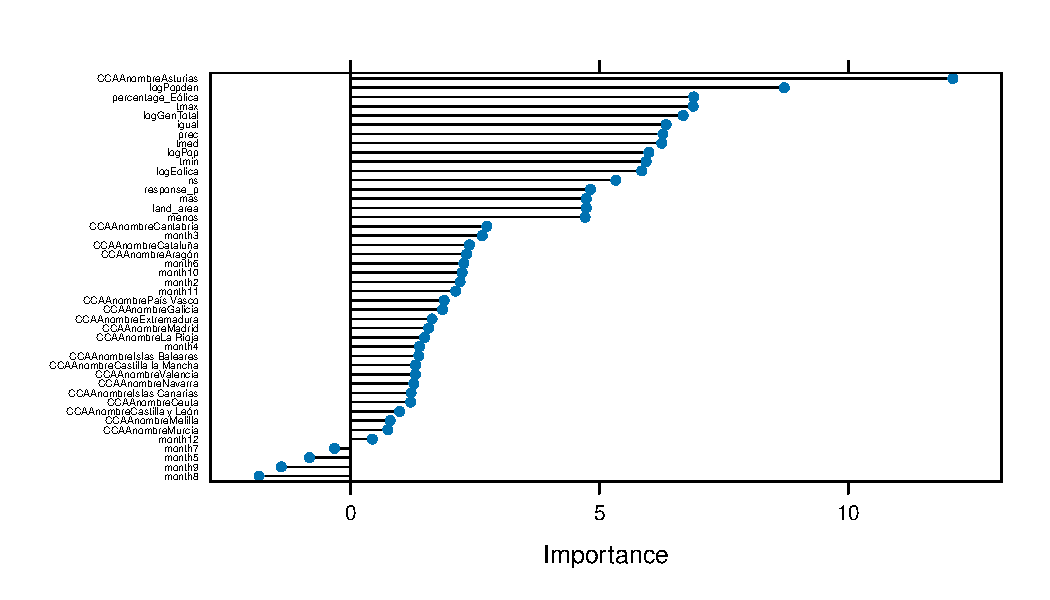
\includegraphics{Thesis-Report-draft1_files/figure-pdf/unnamed-chunk-3-1.pdf}

}

\end{figure}

\begin{Shaded}
\begin{Highlighting}[]
\FunctionTok{ggsave}\NormalTok{(}\AttributeTok{filename =} \StringTok{"cor\_plot.pdf"}\NormalTok{, cor\_plot, }\AttributeTok{width =} \DecValTok{9}\NormalTok{, }\AttributeTok{height =} \DecValTok{7}\NormalTok{, }\AttributeTok{units =} \StringTok{"in"}\NormalTok{ )}
\end{Highlighting}
\end{Shaded}

\hypertarget{linear-models}{%
\section{Linear Models}\label{linear-models}}

Initial linear regression models were developed to explore the impact of
wind energy and population density on energy intensity. The results
suggested a significant positive relationship between log-transformed
wind energy and energy intensity.

\begin{Shaded}
\begin{Highlighting}[]
\NormalTok{month\_plot }\OtherTok{\textless{}{-}}\NormalTok{ agg\_data2022 }\SpecialCharTok{|\textgreater{}} 
  \FunctionTok{ggplot}\NormalTok{(}\FunctionTok{aes}\NormalTok{(}\AttributeTok{y =}\NormalTok{ energy\_int, }\AttributeTok{x =}\NormalTok{ logEolica, }\AttributeTok{color =}\NormalTok{ month)) }\SpecialCharTok{+} 
  \FunctionTok{geom\_line}\NormalTok{(}\AttributeTok{alpha =}\NormalTok{ .}\DecValTok{1}\NormalTok{) }\SpecialCharTok{+} \FunctionTok{geom\_point}\NormalTok{(}\AttributeTok{alpha =}\NormalTok{ .}\DecValTok{1}\NormalTok{)}\SpecialCharTok{+} 
  \FunctionTok{geom\_smooth}\NormalTok{(}\AttributeTok{method =} \StringTok{"glm"}\NormalTok{, }\AttributeTok{se =}\NormalTok{ T) }\SpecialCharTok{+}
  \FunctionTok{labs}\NormalTok{(}
  \CommentTok{\#  title = "Mean energy intensity not significantly different across months"}
\NormalTok{  ) }

\FunctionTok{ggsave}\NormalTok{(}\AttributeTok{filename =} \StringTok{"month{-}plot.pdf"}\NormalTok{, month\_plot, }\AttributeTok{width =} \DecValTok{7}\NormalTok{, }\AttributeTok{height =} \DecValTok{4}\NormalTok{, }\AttributeTok{units =} \StringTok{"in"}\NormalTok{)}
\end{Highlighting}
\end{Shaded}

\begin{Shaded}
\begin{Highlighting}[]
\NormalTok{kableExtra}\SpecialCharTok{::}\FunctionTok{kbl}\NormalTok{(}\FunctionTok{anova}\NormalTok{(aov\_0, aov\_1, aov\_2, aov\_3, aov\_ccaa),}
                \AttributeTok{format =} \StringTok{"latex"}\NormalTok{, }\AttributeTok{row.names =}\NormalTok{ T, }\AttributeTok{caption =} \StringTok{"Analysis of Variance Table"}\NormalTok{,}
\NormalTok{        )}
\end{Highlighting}
\end{Shaded}

\begin{table}

\caption{Analysis of Variance Table}
\centering
\begin{tabular}[t]{l|r|r|r|r|r|r}
\hline
  & Res.Df & RSS & Df & Sum of Sq & F & Pr(>F)\\
\hline
1 & 216 & 5245.1719 & NA & NA & NA & NA\\
\hline
2 & 204 & 2791.8502 & 12 & 2453.3217 & 143.20372 & 0\\
\hline
3 & 204 & 4803.2537 & 0 & -2011.4036 & NA & NA\\
\hline
4 & 198 & 282.6729 & 6 & 4520.5809 & 527.74489 & 0\\
\hline
5 & 209 & 480.0623 & -11 & -197.3894 & 12.56933 & 0\\
\hline
\end{tabular}
\end{table}

\begin{Shaded}
\begin{Highlighting}[]
\NormalTok{for\_tune\_plot }\OtherTok{\textless{}{-}} \FunctionTok{plot}\NormalTok{(for\_tune, }\AttributeTok{metric =} \StringTok{"Rsquared"}\NormalTok{)}

\FunctionTok{coef}\NormalTok{(for\_tune}\SpecialCharTok{$}\NormalTok{finalModel, }\DecValTok{3}\NormalTok{)}
\end{Highlighting}
\end{Shaded}

\begin{verbatim}
NULL
\end{verbatim}

\begin{Shaded}
\begin{Highlighting}[]
\FunctionTok{coef}\NormalTok{(for\_tune}\SpecialCharTok{$}\NormalTok{finalModel, }\DecValTok{6}\NormalTok{)}
\end{Highlighting}
\end{Shaded}

\begin{verbatim}
NULL
\end{verbatim}

\hypertarget{mixed-models}{%
\section{Mixed Models}\label{mixed-models}}

Mixed-effects models were employed to account for the hierarchical
structure of the data, with CCAA and month as random effects. These
models provided a better fit compared to simple linear models.

\begin{Shaded}
\begin{Highlighting}[]
\NormalTok{lmer\_basic}
\end{Highlighting}
\end{Shaded}

\begin{verbatim}
Linear mixed model fit by REML ['lmerMod']
Formula: energy_int ~ logEolica + percentage_Eólica + (1 | CCAAnombre) +  
    (1 | month)
   Data: agg_data2022
REML criterion at convergence: 849.3986
Random effects:
 Groups     Name        Std.Dev.
 CCAAnombre (Intercept) 5.316   
 month      (Intercept) 0.915   
 Residual               1.188   
Number of obs: 228, groups:  CCAAnombre, 19; month, 12
Fixed Effects:
      (Intercept)          logEolica  percentage_Eólica  
          17.9239            -0.2607            -1.0500  
\end{verbatim}

\hypertarget{random-forest}{%
\section{Random Forest}\label{random-forest}}

Random forest models were used to capture non-linear relationships and
interactions between variables. The models indicated that certain
regions, particularly Asturias, significantly influenced energy
intensity.

I decided to run a \emph{Random Forest} model without a variable for
CCAA. This removal should show us which variables are important to
predict energy intensity, without directly asking, ``Which autonomous
community is this?'' Although one possibility would be only keep the
binary dummy variable for when CCAA is equal to Asturias.

I also removed \texttt{month} because it has not shown to be important
without CCAA involved.

This shrunken model with fewer explanatory variables had somewhat
similar results. The most important variable was if the CCAA was
Asturias. That was such a big outlier I had to keep it as a binary
variable. The other most important variables were average temperature
and the survey results for \texttt{igual}.

\begin{Shaded}
\begin{Highlighting}[]
\NormalTok{partial\_ccaa }\OtherTok{\textless{}{-}} \FunctionTok{partial}\NormalTok{(rf\_tune, }\AttributeTok{pred.var =} \StringTok{"CCAAnombre"}\NormalTok{, }\AttributeTok{plot =}\NormalTok{ F) }\SpecialCharTok{|\textgreater{}} 
  \FunctionTok{ggplot}\NormalTok{(}\FunctionTok{aes}\NormalTok{(}\AttributeTok{x =}\NormalTok{ yhat, }\AttributeTok{y =}\NormalTok{ CCAAnombre, }\AttributeTok{xmin =} \DecValTok{0}\NormalTok{, }\AttributeTok{xmax =}\NormalTok{ yhat)) }\SpecialCharTok{+}
  \FunctionTok{geom\_linerange}\NormalTok{(}\AttributeTok{color =} \StringTok{"gray75"}\NormalTok{, }\AttributeTok{linetype =} \StringTok{"dashed"}\NormalTok{) }\SpecialCharTok{+}
  \FunctionTok{geom\_point}\NormalTok{(}\AttributeTok{color =} \StringTok{"\#000066"}\NormalTok{) }\SpecialCharTok{+} \CommentTok{\# xlim(c(15,21)) +}
  \FunctionTok{labs}\NormalTok{(}\AttributeTok{y =} \ConstantTok{NULL}\NormalTok{) }\SpecialCharTok{+} \FunctionTok{scale\_x\_continuous}\NormalTok{(}\AttributeTok{oob =}\NormalTok{ scales}\SpecialCharTok{::}\NormalTok{squish, }\AttributeTok{limits =} \FunctionTok{c}\NormalTok{(}\DecValTok{14}\NormalTok{,}\DecValTok{21}\NormalTok{))}
\FunctionTok{ggsave}\NormalTok{(partial\_ccaa, }\AttributeTok{filename =} \StringTok{"partial\_CCAA.pdf"}\NormalTok{, }\AttributeTok{width =} \DecValTok{4}\NormalTok{, }\AttributeTok{height =} \DecValTok{5}\NormalTok{, }\AttributeTok{units =} \StringTok{"in"}\NormalTok{ )}
\end{Highlighting}
\end{Shaded}

\hypertarget{model-2}{%
\subsection{Model \#2}\label{model-2}}

\begin{Shaded}
\begin{Highlighting}[]
\NormalTok{var\_imp }\OtherTok{\textless{}{-}} \FunctionTok{varImp}\NormalTok{(rf\_tune\_noCCAA, }\AttributeTok{scale =}\NormalTok{ F)}
\NormalTok{rf2\_varImp }\OtherTok{\textless{}{-}} \FunctionTok{data.frame}\NormalTok{(}
  \AttributeTok{var   =} \FunctionTok{row.names}\NormalTok{(var\_imp}\SpecialCharTok{$}\NormalTok{importance),}
  \AttributeTok{importance =}\NormalTok{ var\_imp}\SpecialCharTok{$}\NormalTok{importance[}\DecValTok{1}\NormalTok{]}
\NormalTok{)}
\NormalTok{rf2\_varImp\_plot }\OtherTok{\textless{}{-}}\NormalTok{ rf2\_varImp }\SpecialCharTok{|\textgreater{}} 
  \FunctionTok{ggplot}\NormalTok{(}\FunctionTok{aes}\NormalTok{(}\AttributeTok{x =}\NormalTok{ Overall, }\AttributeTok{xmin =} \DecValTok{0}\NormalTok{, }\AttributeTok{xmax =}\NormalTok{ Overall, }
             \AttributeTok{y =} \FunctionTok{reorder}\NormalTok{(var, Overall))) }\SpecialCharTok{+}
  \FunctionTok{geom\_linerange}\NormalTok{() }\SpecialCharTok{+} \FunctionTok{geom\_point}\NormalTok{(}\AttributeTok{color =} \StringTok{"\#000066"}\NormalTok{) }\SpecialCharTok{+} 
  \FunctionTok{geom\_vline}\NormalTok{(}\AttributeTok{xintercept =} \DecValTok{0}\NormalTok{) }\SpecialCharTok{+} 
  \FunctionTok{labs}\NormalTok{(}\AttributeTok{y =} \ConstantTok{NULL}\NormalTok{, }\AttributeTok{x =} \StringTok{"Importance"}\NormalTok{)}

\FunctionTok{ggsave}\NormalTok{(}\StringTok{"rf2\_varImp\_plot.pdf"}\NormalTok{, rf2\_varImp\_plot, }\AttributeTok{width =} \DecValTok{9}\NormalTok{, }\AttributeTok{height =} \DecValTok{3}\NormalTok{, }\AttributeTok{units =} \StringTok{"in"}\NormalTok{)}
\end{Highlighting}
\end{Shaded}

\begin{Shaded}
\begin{Highlighting}[]
\NormalTok{var\_imp }\OtherTok{\textless{}{-}} \FunctionTok{varImp}\NormalTok{(rf\_tune, }\AttributeTok{scale =}\NormalTok{ F)}
\NormalTok{rf1\_varImp }\OtherTok{\textless{}{-}} \FunctionTok{data.frame}\NormalTok{(}
  \AttributeTok{var   =} \FunctionTok{row.names}\NormalTok{(var\_imp}\SpecialCharTok{$}\NormalTok{importance),}
  \AttributeTok{importance =}\NormalTok{ var\_imp}\SpecialCharTok{$}\NormalTok{importance[}\DecValTok{1}\NormalTok{]}
\NormalTok{)}
\NormalTok{rf1\_varImp\_plot }\OtherTok{\textless{}{-}}\NormalTok{ rf1\_varImp }\SpecialCharTok{|\textgreater{}} 
  \FunctionTok{ggplot}\NormalTok{(}\FunctionTok{aes}\NormalTok{(}\AttributeTok{x =}\NormalTok{ Overall, }\AttributeTok{xmin =} \DecValTok{0}\NormalTok{, }\AttributeTok{xmax =}\NormalTok{ Overall, }
             \AttributeTok{y =} \FunctionTok{reorder}\NormalTok{(var, Overall))) }\SpecialCharTok{+}
  \FunctionTok{geom\_linerange}\NormalTok{() }\SpecialCharTok{+} \FunctionTok{geom\_point}\NormalTok{(}\AttributeTok{color =} \StringTok{"\#000066"}\NormalTok{) }\SpecialCharTok{+} 
  \FunctionTok{geom\_vline}\NormalTok{(}\AttributeTok{xintercept =} \DecValTok{0}\NormalTok{) }\SpecialCharTok{+} 
  \FunctionTok{labs}\NormalTok{(}\AttributeTok{y =} \ConstantTok{NULL}\NormalTok{, }\AttributeTok{x =} \StringTok{"Importance"}\NormalTok{)}

\FunctionTok{ggsave}\NormalTok{(}\StringTok{"rf1\_varImp\_plot.pdf"}\NormalTok{, rf1\_varImp\_plot, }\AttributeTok{width =} \DecValTok{7}\NormalTok{, }\AttributeTok{height =} \DecValTok{7}\NormalTok{, }\AttributeTok{units =} \StringTok{"in"}\NormalTok{)}
\end{Highlighting}
\end{Shaded}

\begin{Shaded}
\begin{Highlighting}[]
\NormalTok{var\_imp }\OtherTok{\textless{}{-}} \FunctionTok{varImp}\NormalTok{(rf\_tune\_small, }\AttributeTok{scale =}\NormalTok{ F)}
\NormalTok{rfsmall\_varImp }\OtherTok{\textless{}{-}} \FunctionTok{data.frame}\NormalTok{(}
  \AttributeTok{var   =} \FunctionTok{row.names}\NormalTok{(var\_imp}\SpecialCharTok{$}\NormalTok{importance),}
  \AttributeTok{importance =}\NormalTok{ var\_imp}\SpecialCharTok{$}\NormalTok{importance[}\DecValTok{1}\NormalTok{]}
\NormalTok{)}
\NormalTok{rfsmall\_varImp\_plot }\OtherTok{\textless{}{-}}\NormalTok{ rfsmall\_varImp }\SpecialCharTok{|\textgreater{}} 
  \FunctionTok{ggplot}\NormalTok{(}\FunctionTok{aes}\NormalTok{(}\AttributeTok{x =}\NormalTok{ Overall, }\AttributeTok{xmin =} \DecValTok{0}\NormalTok{, }\AttributeTok{xmax =}\NormalTok{ Overall, }
             \AttributeTok{y =} \FunctionTok{reorder}\NormalTok{(var, Overall))) }\SpecialCharTok{+}
  \FunctionTok{geom\_linerange}\NormalTok{() }\SpecialCharTok{+} \FunctionTok{geom\_point}\NormalTok{(}\AttributeTok{color =} \StringTok{"\#000066"}\NormalTok{) }\SpecialCharTok{+} 
  \FunctionTok{geom\_vline}\NormalTok{(}\AttributeTok{xintercept =} \DecValTok{0}\NormalTok{) }\SpecialCharTok{+} 
  \FunctionTok{labs}\NormalTok{(}\AttributeTok{y =} \ConstantTok{NULL}\NormalTok{, }\AttributeTok{x =} \StringTok{"Importance"}\NormalTok{)}

\FunctionTok{ggsave}\NormalTok{(}\StringTok{"rfsmall\_varImp\_plot.pdf"}\NormalTok{, rfsmall\_varImp\_plot, }\AttributeTok{width =} \DecValTok{7}\NormalTok{, }\AttributeTok{height =} \DecValTok{2}\NormalTok{, }\AttributeTok{units =} \StringTok{"in"}\NormalTok{)}
\end{Highlighting}
\end{Shaded}

\begin{Shaded}
\begin{Highlighting}[]
\FunctionTok{library}\NormalTok{(patchwork)}

\NormalTok{partial\_1 }\OtherTok{\textless{}{-}} \FunctionTok{partial}\NormalTok{(rf\_tune\_small, }\AttributeTok{pred.var =} \StringTok{"Eolica"}\NormalTok{, }\AttributeTok{plot =}\NormalTok{ F) }\SpecialCharTok{|\textgreater{}} 
  \FunctionTok{ggplot}\NormalTok{(}\FunctionTok{aes}\NormalTok{(}\AttributeTok{y =}\NormalTok{ yhat, }\AttributeTok{x =}\NormalTok{ Eolica)) }\SpecialCharTok{+} \FunctionTok{geom\_line}\NormalTok{() }\SpecialCharTok{+}
  \FunctionTok{geom\_point}\NormalTok{(}\AttributeTok{color =} \StringTok{"\#000066"}\NormalTok{) }\SpecialCharTok{+} \CommentTok{\#ylim(c(13,18))+}
  \FunctionTok{scale\_x\_continuous}\NormalTok{(}\AttributeTok{labels =}\NormalTok{ scales}\SpecialCharTok{::}\FunctionTok{label\_number}\NormalTok{(}\AttributeTok{scale\_cut =}\NormalTok{ scales}\SpecialCharTok{::}\FunctionTok{cut\_long\_scale}\NormalTok{()))}
\NormalTok{partial\_2 }\OtherTok{\textless{}{-}} \FunctionTok{partial}\NormalTok{(rf\_tune\_small, }\AttributeTok{pred.var =} \StringTok{"prec"}\NormalTok{, }\AttributeTok{plot =}\NormalTok{ F) }\SpecialCharTok{|\textgreater{}} 
  \FunctionTok{ggplot}\NormalTok{(}\FunctionTok{aes}\NormalTok{(}\AttributeTok{y =}\NormalTok{ yhat, }\AttributeTok{x =}\NormalTok{ prec)) }\SpecialCharTok{+} \FunctionTok{geom\_line}\NormalTok{() }\SpecialCharTok{+} \CommentTok{\#ylim(c(13,18)) +}
  \FunctionTok{geom\_point}\NormalTok{(}\AttributeTok{color =} \StringTok{"\#000066"}\NormalTok{) }
\NormalTok{partial\_3 }\OtherTok{\textless{}{-}} \FunctionTok{partial}\NormalTok{(rf\_tune\_small, }\AttributeTok{pred.var =} \StringTok{"GenTotal"}\NormalTok{, }\AttributeTok{plot =}\NormalTok{ F) }\SpecialCharTok{|\textgreater{}} 
  \FunctionTok{ggplot}\NormalTok{(}\FunctionTok{aes}\NormalTok{(}\AttributeTok{y =}\NormalTok{ yhat, }\AttributeTok{x =}\NormalTok{ GenTotal)) }\SpecialCharTok{+}\FunctionTok{geom\_line}\NormalTok{() }\SpecialCharTok{+}
  \FunctionTok{geom\_point}\NormalTok{(}\AttributeTok{color =} \StringTok{"\#000066"}\NormalTok{) }\SpecialCharTok{+} \CommentTok{\#ylim(c(13,18))+}
  \FunctionTok{scale\_x\_continuous}\NormalTok{(}\AttributeTok{labels =}\NormalTok{ scales}\SpecialCharTok{::}\FunctionTok{label\_number}\NormalTok{(}\AttributeTok{scale\_cut =}\NormalTok{ scales}\SpecialCharTok{::}\FunctionTok{cut\_long\_scale}\NormalTok{()))}
\NormalTok{partial\_4 }\OtherTok{\textless{}{-}} \FunctionTok{partial}\NormalTok{(rf\_tune\_small, }\AttributeTok{pred.var =} \StringTok{"pop"}\NormalTok{, }\AttributeTok{plot =}\NormalTok{ F) }\SpecialCharTok{|\textgreater{}} 
  \FunctionTok{ggplot}\NormalTok{(}\FunctionTok{aes}\NormalTok{(}\AttributeTok{y =}\NormalTok{ yhat, }\AttributeTok{x =}\NormalTok{ pop)) }\SpecialCharTok{+} \FunctionTok{geom\_line}\NormalTok{() }\SpecialCharTok{+}
  \FunctionTok{geom\_point}\NormalTok{(}\AttributeTok{color =} \StringTok{"\#000066"}\NormalTok{)}\SpecialCharTok{+}\CommentTok{\# ylim(c(13,18))+}
  \FunctionTok{scale\_x\_continuous}\NormalTok{(}\AttributeTok{labels =}\NormalTok{ scales}\SpecialCharTok{::}\FunctionTok{label\_number}\NormalTok{(}\AttributeTok{scale\_cut =}\NormalTok{ scales}\SpecialCharTok{::}\FunctionTok{cut\_long\_scale}\NormalTok{())) }
\NormalTok{partial\_5 }\OtherTok{\textless{}{-}} \FunctionTok{partial}\NormalTok{(rf\_tune\_small, }\AttributeTok{pred.var =} \StringTok{"percentage\_Eólica"}\NormalTok{, }\AttributeTok{plot =}\NormalTok{ F) }\SpecialCharTok{|\textgreater{}} 
  \FunctionTok{ggplot}\NormalTok{(}\FunctionTok{aes}\NormalTok{(}\AttributeTok{y =}\NormalTok{ yhat, }\AttributeTok{x =}\NormalTok{ percentage\_Eólica)) }\SpecialCharTok{+} \FunctionTok{geom\_line}\NormalTok{() }\SpecialCharTok{+}
  \FunctionTok{geom\_point}\NormalTok{(}\AttributeTok{color =} \StringTok{"\#000066"}\NormalTok{)}\SpecialCharTok{+} \CommentTok{\# ylim(c(13,18))+}
  \FunctionTok{scale\_x\_continuous}\NormalTok{(}\AttributeTok{labels =}\NormalTok{ scales}\SpecialCharTok{::}\FunctionTok{label\_percent}\NormalTok{() )}

\NormalTok{partial\_6 }\OtherTok{\textless{}{-}} \FunctionTok{partial}\NormalTok{(rf\_tune\_small, }\AttributeTok{pred.var =} \StringTok{"mas"}\NormalTok{, }\AttributeTok{plot =}\NormalTok{ F) }\SpecialCharTok{|\textgreater{}} 
  \FunctionTok{ggplot}\NormalTok{(}\FunctionTok{aes}\NormalTok{(}\AttributeTok{y =}\NormalTok{ yhat, }\AttributeTok{x =}\NormalTok{ mas)) }\SpecialCharTok{+} \FunctionTok{geom\_line}\NormalTok{() }\SpecialCharTok{+}
  \FunctionTok{geom\_point}\NormalTok{(}\AttributeTok{color =} \StringTok{"\#000066"}\NormalTok{)}\SpecialCharTok{+} \CommentTok{\#ylim(c(13,18))+}
  \FunctionTok{scale\_x\_continuous}\NormalTok{(}\AttributeTok{labels =}\NormalTok{ scales}\SpecialCharTok{::}\FunctionTok{label\_percent}\NormalTok{() ) }

\NormalTok{partial\_small }\OtherTok{\textless{}{-}}\NormalTok{ (partial\_1 }\SpecialCharTok{+}\NormalTok{ partial\_3)}\SpecialCharTok{/}\NormalTok{(partial\_2 }\SpecialCharTok{+}\NormalTok{ partial\_4) }\SpecialCharTok{/}\NormalTok{(partial\_5 }\SpecialCharTok{+}\NormalTok{ partial\_6)}

\FunctionTok{ggsave}\NormalTok{(partial\_small, }\AttributeTok{filename =} \StringTok{"partial\_small.pdf"}\NormalTok{, }\AttributeTok{width =} \DecValTok{7}\NormalTok{, }\AttributeTok{height =} \DecValTok{7}\NormalTok{, }\AttributeTok{units =} \StringTok{"in"}\NormalTok{ )}
\end{Highlighting}
\end{Shaded}

\hypertarget{regularized-regression}{%
\section{Regularized Regression}\label{regularized-regression}}

Elastic net regularization was applied to manage multicollinearity among
predictors. This approach highlighted the importance of specific
variables, such as population densityand total electricity generated, in
predicting energy intensity.

\begin{Shaded}
\begin{Highlighting}[]
\NormalTok{var\_imp }\OtherTok{\textless{}{-}} \FunctionTok{varImp}\NormalTok{(glmnet\_tune, }\AttributeTok{scale =}\NormalTok{ F)}
\NormalTok{glmnet\_varImp }\OtherTok{\textless{}{-}} \FunctionTok{data.frame}\NormalTok{(}
  \AttributeTok{var   =} \FunctionTok{row.names}\NormalTok{(var\_imp}\SpecialCharTok{$}\NormalTok{importance),}
  \AttributeTok{importance =}\NormalTok{ var\_imp}\SpecialCharTok{$}\NormalTok{importance[}\DecValTok{1}\NormalTok{]}
\NormalTok{)}
\NormalTok{glmnet\_varImp\_plot }\OtherTok{\textless{}{-}}\NormalTok{ glmnet\_varImp }\SpecialCharTok{|\textgreater{}} 
  \FunctionTok{ggplot}\NormalTok{(}\FunctionTok{aes}\NormalTok{(}\AttributeTok{x =}\NormalTok{ Overall, }\AttributeTok{xmin =} \DecValTok{0}\NormalTok{, }\AttributeTok{xmax =}\NormalTok{ Overall, }
             \AttributeTok{y =} \FunctionTok{reorder}\NormalTok{(var, Overall))) }\SpecialCharTok{+}
  \FunctionTok{geom\_linerange}\NormalTok{() }\SpecialCharTok{+} \FunctionTok{geom\_point}\NormalTok{(}\AttributeTok{color =} \StringTok{"\#000066"}\NormalTok{) }\SpecialCharTok{+} 
  \FunctionTok{geom\_vline}\NormalTok{(}\AttributeTok{xintercept =} \DecValTok{0}\NormalTok{) }\SpecialCharTok{+} 
  \FunctionTok{labs}\NormalTok{(}\AttributeTok{y =} \ConstantTok{NULL}\NormalTok{, }\AttributeTok{x =} \StringTok{"Importance"}\NormalTok{) }\SpecialCharTok{+} \FunctionTok{theme}\NormalTok{(}\AttributeTok{plot.background =} \FunctionTok{element\_rect}\NormalTok{(}\AttributeTok{fill =} \StringTok{"gray75"}\NormalTok{))}

\FunctionTok{ggsave}\NormalTok{(}\StringTok{"glmnet\_varImp\_plot.pdf"}\NormalTok{, glmnet\_varImp\_plot, }\AttributeTok{width =} \DecValTok{7}\NormalTok{, }\AttributeTok{height =} \DecValTok{5}\NormalTok{, }\AttributeTok{units =} \StringTok{"in"}\NormalTok{)}
\end{Highlighting}
\end{Shaded}

\begin{Shaded}
\begin{Highlighting}[]
\NormalTok{partial\_1 }\OtherTok{\textless{}{-}} \FunctionTok{partial}\NormalTok{(rf\_tune\_small, }\AttributeTok{pred.var =} \StringTok{"Eolica"}\NormalTok{, }\AttributeTok{plot =}\NormalTok{ F) }\SpecialCharTok{|\textgreater{}} 
  \FunctionTok{ggplot}\NormalTok{(}\FunctionTok{aes}\NormalTok{(}\AttributeTok{y =}\NormalTok{ yhat, }\AttributeTok{x =}\NormalTok{ Eolica)) }\SpecialCharTok{+} \FunctionTok{geom\_line}\NormalTok{() }\SpecialCharTok{+}
  \FunctionTok{geom\_point}\NormalTok{(}\AttributeTok{color =} \StringTok{"\#000066"}\NormalTok{) }\SpecialCharTok{+} \CommentTok{\#ylim(c(13,18))+}
  \FunctionTok{scale\_x\_continuous}\NormalTok{(}\AttributeTok{labels =}\NormalTok{ scales}\SpecialCharTok{::}\FunctionTok{label\_number}\NormalTok{(}\AttributeTok{scale\_cut =}\NormalTok{ scales}\SpecialCharTok{::}\FunctionTok{cut\_long\_scale}\NormalTok{()))}
\NormalTok{partial\_2 }\OtherTok{\textless{}{-}} \FunctionTok{partial}\NormalTok{(rf\_tune\_small, }\AttributeTok{pred.var =} \StringTok{"prec"}\NormalTok{, }\AttributeTok{plot =}\NormalTok{ F) }\SpecialCharTok{|\textgreater{}} 
  \FunctionTok{ggplot}\NormalTok{(}\FunctionTok{aes}\NormalTok{(}\AttributeTok{y =}\NormalTok{ yhat, }\AttributeTok{x =}\NormalTok{ prec)) }\SpecialCharTok{+} \FunctionTok{geom\_line}\NormalTok{() }\SpecialCharTok{+} \CommentTok{\#ylim(c(13,18)) +}
  \FunctionTok{geom\_point}\NormalTok{(}\AttributeTok{color =} \StringTok{"\#000066"}\NormalTok{) }
\NormalTok{partial\_3 }\OtherTok{\textless{}{-}} \FunctionTok{partial}\NormalTok{(rf\_tune\_small, }\AttributeTok{pred.var =} \StringTok{"GenTotal"}\NormalTok{, }\AttributeTok{plot =}\NormalTok{ F) }\SpecialCharTok{|\textgreater{}} 
  \FunctionTok{ggplot}\NormalTok{(}\FunctionTok{aes}\NormalTok{(}\AttributeTok{y =}\NormalTok{ yhat, }\AttributeTok{x =}\NormalTok{ GenTotal)) }\SpecialCharTok{+}\FunctionTok{geom\_line}\NormalTok{() }\SpecialCharTok{+}
  \FunctionTok{geom\_point}\NormalTok{(}\AttributeTok{color =} \StringTok{"\#000066"}\NormalTok{) }\SpecialCharTok{+} \CommentTok{\#ylim(c(13,18))+}
  \FunctionTok{scale\_x\_continuous}\NormalTok{(}\AttributeTok{labels =}\NormalTok{ scales}\SpecialCharTok{::}\FunctionTok{label\_number}\NormalTok{(}\AttributeTok{scale\_cut =}\NormalTok{ scales}\SpecialCharTok{::}\FunctionTok{cut\_long\_scale}\NormalTok{()))}
\NormalTok{partial\_4 }\OtherTok{\textless{}{-}} \FunctionTok{partial}\NormalTok{(rf\_tune\_small, }\AttributeTok{pred.var =} \StringTok{"pop"}\NormalTok{, }\AttributeTok{plot =}\NormalTok{ F) }\SpecialCharTok{|\textgreater{}} 
  \FunctionTok{ggplot}\NormalTok{(}\FunctionTok{aes}\NormalTok{(}\AttributeTok{y =}\NormalTok{ yhat, }\AttributeTok{x =}\NormalTok{ pop)) }\SpecialCharTok{+} \FunctionTok{geom\_line}\NormalTok{() }\SpecialCharTok{+}
  \FunctionTok{geom\_point}\NormalTok{(}\AttributeTok{color =} \StringTok{"\#000066"}\NormalTok{)}\SpecialCharTok{+}\CommentTok{\# ylim(c(13,18))+}
  \FunctionTok{scale\_x\_continuous}\NormalTok{(}\AttributeTok{labels =}\NormalTok{ scales}\SpecialCharTok{::}\FunctionTok{label\_number}\NormalTok{(}\AttributeTok{scale\_cut =}\NormalTok{ scales}\SpecialCharTok{::}\FunctionTok{cut\_long\_scale}\NormalTok{())) }
\NormalTok{partial\_5 }\OtherTok{\textless{}{-}} \FunctionTok{partial}\NormalTok{(rf\_tune\_small, }\AttributeTok{pred.var =} \StringTok{"percentage\_Eólica"}\NormalTok{, }\AttributeTok{plot =}\NormalTok{ F) }\SpecialCharTok{|\textgreater{}} 
  \FunctionTok{ggplot}\NormalTok{(}\FunctionTok{aes}\NormalTok{(}\AttributeTok{y =}\NormalTok{ yhat, }\AttributeTok{x =}\NormalTok{ percentage\_Eólica)) }\SpecialCharTok{+} \FunctionTok{geom\_line}\NormalTok{() }\SpecialCharTok{+}
  \FunctionTok{geom\_point}\NormalTok{(}\AttributeTok{color =} \StringTok{"\#000066"}\NormalTok{)}\SpecialCharTok{+} \CommentTok{\# ylim(c(13,18))+}
  \FunctionTok{scale\_x\_continuous}\NormalTok{(}\AttributeTok{labels =}\NormalTok{ scales}\SpecialCharTok{::}\FunctionTok{label\_percent}\NormalTok{() )}

\NormalTok{partial\_6 }\OtherTok{\textless{}{-}} \FunctionTok{partial}\NormalTok{(rf\_tune\_small, }\AttributeTok{pred.var =} \StringTok{"mas"}\NormalTok{, }\AttributeTok{plot =}\NormalTok{ F) }\SpecialCharTok{|\textgreater{}} 
  \FunctionTok{ggplot}\NormalTok{(}\FunctionTok{aes}\NormalTok{(}\AttributeTok{y =}\NormalTok{ yhat, }\AttributeTok{x =}\NormalTok{ mas)) }\SpecialCharTok{+} \FunctionTok{geom\_line}\NormalTok{() }\SpecialCharTok{+}
  \FunctionTok{geom\_point}\NormalTok{(}\AttributeTok{color =} \StringTok{"\#000066"}\NormalTok{)}\SpecialCharTok{+} \CommentTok{\#ylim(c(13,18))+}
  \FunctionTok{scale\_x\_continuous}\NormalTok{(}\AttributeTok{labels =}\NormalTok{ scales}\SpecialCharTok{::}\FunctionTok{label\_percent}\NormalTok{() ) }

\NormalTok{partial\_glmnet }\OtherTok{\textless{}{-}}\NormalTok{ (partial\_1 }\SpecialCharTok{+}\NormalTok{ partial\_3)}\SpecialCharTok{/}\NormalTok{(partial\_2 }\SpecialCharTok{+}\NormalTok{ partial\_4) }\SpecialCharTok{/}\NormalTok{(partial\_5 }\SpecialCharTok{+}\NormalTok{ partial\_6)}

\FunctionTok{ggsave}\NormalTok{(partial\_glmnet, }\AttributeTok{filename =} \StringTok{"partial\_glmnet.pdf"}\NormalTok{, }\AttributeTok{width =} \DecValTok{7}\NormalTok{, }\AttributeTok{height =} \DecValTok{7}\NormalTok{, }\AttributeTok{units =} \StringTok{"in"}\NormalTok{ )}
\end{Highlighting}
\end{Shaded}

\hypertarget{results}{%
\chapter{Results}\label{results}}

\hypertarget{is-month-a-significant-predictor}{%
\section{Is Month a Significant
Predictor?}\label{is-month-a-significant-predictor}}

ANOVA tests were conducted to evaluate whether the month significantly
predicts energy intensity. The results indicated that month alone is not
a significant predictor, but its interaction with other variables, such
as wind energy generation, can influence energy intensity.

\hypertarget{ccaa-as-a-significant-predictor}{%
\section{CCAA as a Significant
Predictor}\label{ccaa-as-a-significant-predictor}}

The analysis showed that CCAA is a significant predictor of energy
intensity. Mixed models incorporating CCAA provided the best fit,
underscoring the importance of regional differences in energy
consumption patterns.

\hypertarget{are-the-survey-results-significant}{%
\section{Are the survey results
significant?}\label{are-the-survey-results-significant}}

\begin{Shaded}
\begin{Highlighting}[]
\NormalTok{z }\OtherTok{\textless{}{-}}  \FloatTok{1.96}
\NormalTok{survey }\SpecialCharTok{|\textgreater{}} 
  \FunctionTok{select}\NormalTok{(CCAAnombre, response\_p, response\_sd, total.y) }\SpecialCharTok{|\textgreater{}} 
  \FunctionTok{mutate}\NormalTok{(}\AttributeTok{moe =}\NormalTok{ z }\SpecialCharTok{*} \FunctionTok{sqrt}\NormalTok{(response\_p }\SpecialCharTok{*}\NormalTok{ (}\DecValTok{1} \SpecialCharTok{{-}}\NormalTok{ response\_p) }\SpecialCharTok{/}\NormalTok{ total.y)) }\SpecialCharTok{|\textgreater{}} \CommentTok{\# calculate margin of error with 95\% conf. level.}
    \FunctionTok{ggplot}\NormalTok{(}\FunctionTok{aes}\NormalTok{(}\AttributeTok{y =} \FunctionTok{reorder}\NormalTok{(CCAAnombre, response\_p), }\AttributeTok{x =}\NormalTok{ response\_p,}
             \AttributeTok{xmax =}\NormalTok{ moe }\SpecialCharTok{+}\NormalTok{ response\_p, }
             \AttributeTok{xmin =}\NormalTok{ response\_p }\SpecialCharTok{{-}}\NormalTok{ moe)) }\SpecialCharTok{+}
  \FunctionTok{geom\_linerange}\NormalTok{(}\AttributeTok{color =} \StringTok{"gray0"}\NormalTok{) }\SpecialCharTok{+}
  \FunctionTok{geom\_point}\NormalTok{(}\AttributeTok{color =} \StringTok{"\#000066"}\NormalTok{) }\SpecialCharTok{+}
  \FunctionTok{labs}\NormalTok{( }
    \AttributeTok{y =} \ConstantTok{NULL}\NormalTok{, }\AttributeTok{x =} \StringTok{"issues\_p"}\NormalTok{,}
    \AttributeTok{caption =} \StringTok{"Data source: CIS"}
\NormalTok{  ) }\SpecialCharTok{+}
  \FunctionTok{scale\_x\_continuous}\NormalTok{(}
    \AttributeTok{labels =}\NormalTok{ scales}\SpecialCharTok{::}\FunctionTok{label\_percent}\NormalTok{(),}
    \AttributeTok{limits =} \FunctionTok{c}\NormalTok{(}\DecValTok{0}\NormalTok{,}\DecValTok{1}\NormalTok{),}
    \AttributeTok{oob =}\NormalTok{ scales}\SpecialCharTok{::}\NormalTok{squish}
\NormalTok{  )  }\SpecialCharTok{+}
  \FunctionTok{theme}\NormalTok{(}
    \AttributeTok{axis.text.y =} \FunctionTok{element\_text}\NormalTok{(}\AttributeTok{size =} \DecValTok{12}\NormalTok{, }\AttributeTok{face =} \StringTok{"bold"}\NormalTok{, }\AttributeTok{color =} \StringTok{"black"}\NormalTok{),}
    \AttributeTok{panel.grid.major.x =} \FunctionTok{element\_line}\NormalTok{(}\AttributeTok{color =} \StringTok{"gray75"}\NormalTok{, }\AttributeTok{linetype =} \StringTok{"dotted"}\NormalTok{),}
    \AttributeTok{panel.grid.minor.x =} \FunctionTok{element\_line}\NormalTok{(}\AttributeTok{color =} \StringTok{"gray75"}\NormalTok{, }\AttributeTok{linetype =} \StringTok{"dotted"}\NormalTok{)}
\NormalTok{  )}
\end{Highlighting}
\end{Shaded}

\begin{figure}[H]

{\centering \includegraphics{Thesis-Report-draft1_files/figure-pdf/response-ccaa-1.pdf}

}

\end{figure}

\begin{Shaded}
\begin{Highlighting}[]
\FunctionTok{ggsave}\NormalTok{(}\AttributeTok{filename =} \StringTok{"issues{-}ccaa.pdf"}\NormalTok{, }\AttributeTok{width =} \DecValTok{7}\NormalTok{, }\AttributeTok{height =} \DecValTok{5}\NormalTok{, }\AttributeTok{units =} \StringTok{"in"}\NormalTok{ )}
\end{Highlighting}
\end{Shaded}

\begin{Shaded}
\begin{Highlighting}[]
\NormalTok{z }\OtherTok{\textless{}{-}}  \FloatTok{1.96}
\NormalTok{survey }\SpecialCharTok{|\textgreater{}} 
  \FunctionTok{select}\NormalTok{(CCAAnombre, mas, menos, igual, total.y) }\SpecialCharTok{|\textgreater{}} 
  \FunctionTok{mutate}\NormalTok{(}\AttributeTok{moe\_mas =}\NormalTok{ z }\SpecialCharTok{*} \FunctionTok{sqrt}\NormalTok{(mas }\SpecialCharTok{*}\NormalTok{ (}\DecValTok{1} \SpecialCharTok{{-}}\NormalTok{ mas) }\SpecialCharTok{/}\NormalTok{ total.y)) }\SpecialCharTok{|\textgreater{}} \CommentTok{\# calculate margin of error with 95\% conf. level.}
    \FunctionTok{ggplot}\NormalTok{(}\FunctionTok{aes}\NormalTok{(}\AttributeTok{y =} \FunctionTok{reorder}\NormalTok{(CCAAnombre, mas), }\AttributeTok{x =}\NormalTok{ mas,}
             \AttributeTok{xmax =}\NormalTok{ moe\_mas }\SpecialCharTok{+}\NormalTok{ mas, }
             \AttributeTok{xmin =}\NormalTok{ mas }\SpecialCharTok{{-}}\NormalTok{ moe\_mas)) }\SpecialCharTok{+}
  \FunctionTok{geom\_linerange}\NormalTok{(}\AttributeTok{color =} \StringTok{"gray0"}\NormalTok{) }\SpecialCharTok{+}
  \FunctionTok{geom\_point}\NormalTok{(}\AttributeTok{color =} \StringTok{"\#000066"}\NormalTok{) }\SpecialCharTok{+}
  \FunctionTok{labs}\NormalTok{( }
    \AttributeTok{y =} \ConstantTok{NULL}\NormalTok{,}
    \AttributeTok{caption =} \StringTok{"Data source: CIS"}
\NormalTok{  ) }\SpecialCharTok{+}
  \FunctionTok{scale\_x\_continuous}\NormalTok{(}
    \AttributeTok{labels =}\NormalTok{ scales}\SpecialCharTok{::}\FunctionTok{label\_percent}\NormalTok{(),}
    \AttributeTok{limits =} \FunctionTok{c}\NormalTok{(}\DecValTok{0}\NormalTok{,}\DecValTok{1}\NormalTok{),}
    \AttributeTok{oob =}\NormalTok{ scales}\SpecialCharTok{::}\NormalTok{squish}
\NormalTok{  )  }\SpecialCharTok{+}
  \FunctionTok{theme}\NormalTok{(}
    \AttributeTok{axis.text.y =} \FunctionTok{element\_text}\NormalTok{(}\AttributeTok{size =} \DecValTok{12}\NormalTok{, }\AttributeTok{face =} \StringTok{"bold"}\NormalTok{, }\AttributeTok{color =} \StringTok{"black"}\NormalTok{),}
    \AttributeTok{panel.grid.major.x =} \FunctionTok{element\_line}\NormalTok{(}\AttributeTok{color =} \StringTok{"gray75"}\NormalTok{, }\AttributeTok{linetype =} \StringTok{"dotted"}\NormalTok{),}
    \AttributeTok{panel.grid.minor.x =} \FunctionTok{element\_line}\NormalTok{(}\AttributeTok{color =} \StringTok{"gray75"}\NormalTok{, }\AttributeTok{linetype =} \StringTok{"dotted"}\NormalTok{)}
\NormalTok{  )}
\end{Highlighting}
\end{Shaded}

\begin{figure}[H]

{\centering \includegraphics{Thesis-Report-draft1_files/figure-pdf/mas-ccaa-1.pdf}

}

\end{figure}

\begin{Shaded}
\begin{Highlighting}[]
\FunctionTok{ggsave}\NormalTok{(}\AttributeTok{filename =} \StringTok{"mas{-}ccaa.pdf"}\NormalTok{, }\AttributeTok{width =} \DecValTok{7}\NormalTok{, }\AttributeTok{height =} \DecValTok{5}\NormalTok{, }\AttributeTok{units =} \StringTok{"in"}\NormalTok{ )}
\end{Highlighting}
\end{Shaded}

\hypertarget{discussion}{%
\chapter{Discussion}\label{discussion}}

\hypertarget{interpretation-of-results}{%
\section{Interpretation of Results}\label{interpretation-of-results}}

The findings suggest that densely populated areas tend to have higher
energy intensity, and increased wind energy generation is associated
with increased energy intensity. This counterintuitive result may be due
to inefficiencies in energy distribution or other regional factors.

\hypertarget{model-comparisons}{%
\section{Model Comparisons}\label{model-comparisons}}

Comparative analysis of different models revealed that mixed models and
random forest approaches provide better predictive performance compared
to simple linear models. The inclusion of regional (CCAA) and temporal
(month) variables improved the models' explanatory power.

\begin{Shaded}
\begin{Highlighting}[]
\NormalTok{comparisons\_Rsquared }\OtherTok{\textless{}{-}}\NormalTok{ stats\_results }\SpecialCharTok{|\textgreater{}} 
  \FunctionTok{mutate}\NormalTok{(}\AttributeTok{Rsq  =} \FunctionTok{paste0}\NormalTok{(}\FunctionTok{round}\NormalTok{(}\DecValTok{100}\SpecialCharTok{*}\NormalTok{Rsquared, }\DecValTok{1}\NormalTok{), }\StringTok{"\%"}\NormalTok{) ) }\SpecialCharTok{|\textgreater{}} 
  \FunctionTok{filter}\NormalTok{(model }\SpecialCharTok{!=} \StringTok{"actual\_2014"}\NormalTok{) }\SpecialCharTok{|\textgreater{}} 
  \FunctionTok{ggplot}\NormalTok{(}\FunctionTok{aes}\NormalTok{(}\AttributeTok{xmax =}\NormalTok{ Rsquared, }\AttributeTok{xmin =} \DecValTok{0}\NormalTok{,}
             \AttributeTok{x =}\NormalTok{ Rsquared, }\AttributeTok{y =}\NormalTok{ model, }\AttributeTok{label =}\NormalTok{ Rsq)) }\SpecialCharTok{+}
  \FunctionTok{geom\_linerange}\NormalTok{(}\AttributeTok{color =} \StringTok{"\#000066"}\NormalTok{) }\SpecialCharTok{+}
  \FunctionTok{geom\_point}\NormalTok{(}\AttributeTok{color =} \StringTok{"\#000066"}\NormalTok{) }\SpecialCharTok{+}
  \FunctionTok{geom\_text}\NormalTok{(}\AttributeTok{nudge\_x =}\NormalTok{ .}\DecValTok{06}\NormalTok{) }\SpecialCharTok{+}
  \FunctionTok{geom\_vline}\NormalTok{(}\AttributeTok{xintercept =} \DecValTok{0}\NormalTok{) }\SpecialCharTok{+}
  \FunctionTok{labs}\NormalTok{(}
    \AttributeTok{y =} \StringTok{"Models"}
\NormalTok{  ) }\SpecialCharTok{+}
  \FunctionTok{scale\_x\_continuous}\NormalTok{(}
    \AttributeTok{labels =}\NormalTok{ scales}\SpecialCharTok{::}\FunctionTok{label\_percent}\NormalTok{(),}
    \AttributeTok{breaks =} \FunctionTok{c}\NormalTok{(}\DecValTok{0}\NormalTok{,.}\DecValTok{2}\NormalTok{,.}\DecValTok{4}\NormalTok{, .}\DecValTok{6}\NormalTok{, .}\DecValTok{8}\NormalTok{, }\DecValTok{1}\NormalTok{), }
    \AttributeTok{limits =} \FunctionTok{c}\NormalTok{(}\DecValTok{0}\NormalTok{,}\DecValTok{1}\NormalTok{)}
\NormalTok{  ) }

\NormalTok{comparisons\_rmse }\OtherTok{\textless{}{-}}\NormalTok{ stats\_results }\SpecialCharTok{|\textgreater{}} 
  \FunctionTok{mutate}\NormalTok{(}\AttributeTok{rmselab  =} \FunctionTok{paste0}\NormalTok{(}\FunctionTok{round}\NormalTok{(RMSE, }\DecValTok{2}\NormalTok{)) ) }\SpecialCharTok{|\textgreater{}} 
  \FunctionTok{filter}\NormalTok{(model }\SpecialCharTok{!=} \StringTok{"actual\_2014"}\NormalTok{) }\SpecialCharTok{|\textgreater{}} 
  \FunctionTok{ggplot}\NormalTok{(}\FunctionTok{aes}\NormalTok{(}\AttributeTok{xmax =}\NormalTok{ RMSE, }\AttributeTok{xmin =} \DecValTok{0}\NormalTok{,}
             \AttributeTok{x =}\NormalTok{ RMSE, }\AttributeTok{y =}\NormalTok{ model, }\AttributeTok{label =}\NormalTok{ rmselab)) }\SpecialCharTok{+}
  \FunctionTok{geom\_linerange}\NormalTok{(}\AttributeTok{color =} \StringTok{"\#000066"}\NormalTok{) }\SpecialCharTok{+}
  \FunctionTok{geom\_point}\NormalTok{(}\AttributeTok{color =} \StringTok{"\#000066"}\NormalTok{) }\SpecialCharTok{+}
  \FunctionTok{geom\_text}\NormalTok{(}\AttributeTok{nudge\_x =}\NormalTok{ .}\DecValTok{3}\NormalTok{) }\SpecialCharTok{+}
  \FunctionTok{geom\_vline}\NormalTok{(}\AttributeTok{xintercept =} \DecValTok{0}\NormalTok{) }\SpecialCharTok{+}
  \FunctionTok{labs}\NormalTok{(}
    \AttributeTok{y =} \ConstantTok{NULL}
\NormalTok{  ) }

\NormalTok{comparisons\_plot }\OtherTok{\textless{}{-}}\NormalTok{ comparisons\_Rsquared }\SpecialCharTok{+}\NormalTok{ comparisons\_rmse }\SpecialCharTok{+}\FunctionTok{plot\_layout}\NormalTok{(}\AttributeTok{widths =} \FunctionTok{c}\NormalTok{(}\FloatTok{0.6}\NormalTok{,}\FloatTok{0.4}\NormalTok{))}

\FunctionTok{ggsave}\NormalTok{(comparisons\_plot, }\AttributeTok{filename =} \StringTok{"comparisons{-}plot.pdf"}\NormalTok{, }\AttributeTok{width =} \DecValTok{10}\NormalTok{, }\AttributeTok{height =} \DecValTok{4}\NormalTok{, }\AttributeTok{units =} \StringTok{"in"}\NormalTok{ )}
\FunctionTok{ggsave}\NormalTok{(comparisons\_Rsquared, }\AttributeTok{filename =} \StringTok{"comparisons{-}rsq.pdf"}\NormalTok{, }\AttributeTok{width =} \DecValTok{7}\NormalTok{, }\AttributeTok{height =} \DecValTok{4}\NormalTok{, }\AttributeTok{units =} \StringTok{"in"}\NormalTok{ )}
\FunctionTok{ggsave}\NormalTok{(comparisons\_rmse, }\AttributeTok{filename =} \StringTok{"comparisons{-}rmse.pdf"}\NormalTok{, }\AttributeTok{width =} \DecValTok{7}\NormalTok{, }\AttributeTok{height =} \DecValTok{4}\NormalTok{, }\AttributeTok{units =} \StringTok{"in"}\NormalTok{ )}
\end{Highlighting}
\end{Shaded}

\hypertarget{conclusion}{%
\chapter{Conclusion}\label{conclusion}}

This study provides insights into the factors influencing energy
intensity across different regions. The results emphasize the importance
of considering regional and temporal variations in energy policy
planning. Future research should explore the underlying causes of the
observed relationships and investigate additional variables that may
impact energy intensity.

\hypertarget{references}{%
\chapter{References}\label{references}}

(Include your references here, formatted according to the required
citation style)

\hypertarget{appendices}{%
\chapter{Appendices}\label{appendices}}

\hypertarget{appendix-a-data-preprocessing-steps}{%
\section{Appendix A: Data Preprocessing
Steps}\label{appendix-a-data-preprocessing-steps}}

\hypertarget{appendix-b-detailed-model-outputs}{%
\section{Appendix B: Detailed Model
Outputs}\label{appendix-b-detailed-model-outputs}}

\hypertarget{appendix-c-additional-figures-and-tables}{%
\section{Appendix C: Additional Figures and
Tables}\label{appendix-c-additional-figures-and-tables}}



\end{document}
